\chapter{Case study and MATLAB simulation implementation}\label{section-case}
In this chapter, an specific example\cite{hovell2017experimental} of tether satellite system is studied. In this case study, the used dynamic model and Proportional-Differentiation controller are the main analysis focuses. At the end, MATLAB simulation is also implemented.

The tether satellite system consists of two satellite and a tether. The two satellites are named as Target Vehicle and Chaser vehicle which means the task of Chaser vehicle is to capture the target vehicle and to de-rotation of the system. In the real case the target vehicle can be space debris which is moving and rotation around Earth under the gravitational force of the Earth. Space debris not only rotates around the Earth, in fact it will also rotate around its body center if any .De-orbiting can be achieved if the energy and angular momentum of space debris consumed.
\begin{figure}[ht]

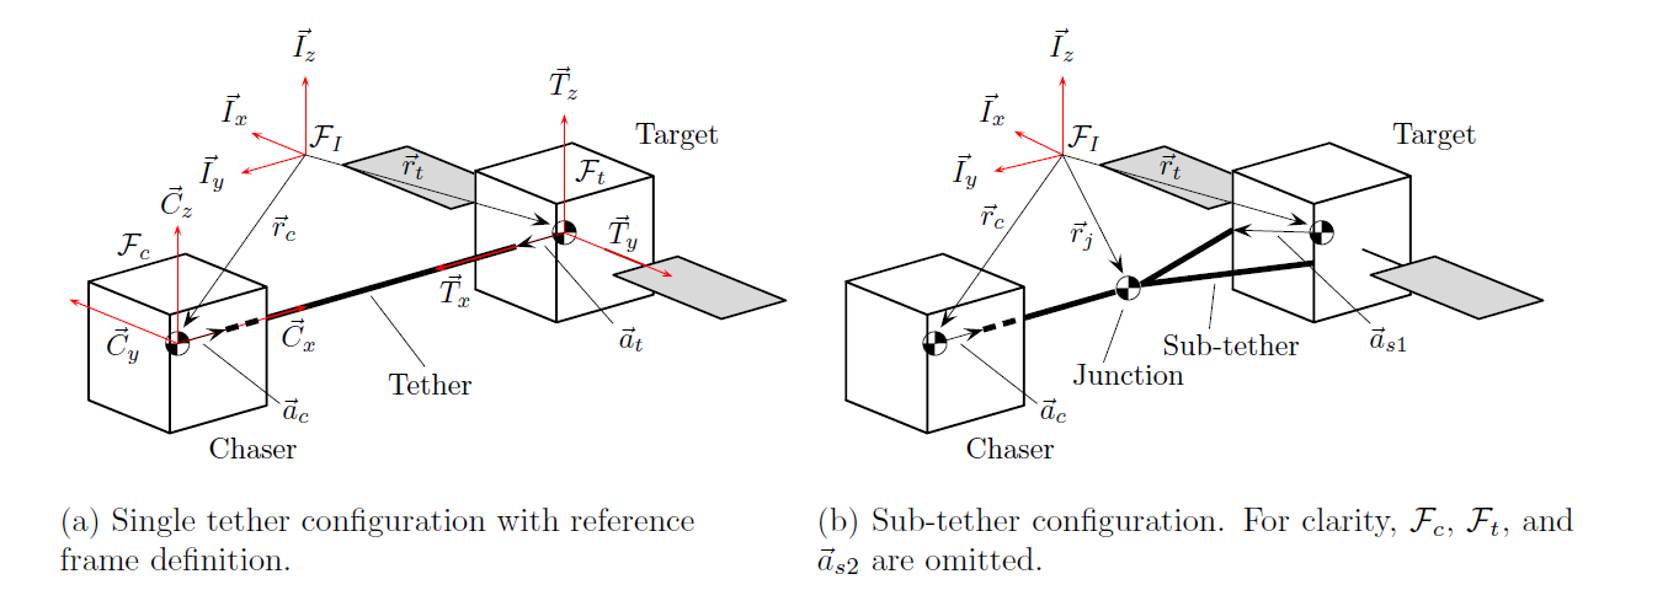
\includegraphics[width=\textwidth]{fig/simulation/ReferenceFrame}
\caption{Reference frame and vector definition for planar dynamics modeling}

\end{figure}
When we let our chaser vehicle connect with target vehicle using tether, the consumption of angular momentum becomes faster and the deorbiting gets quicker.  
So we can say that chaser vehicle plays as a role of active debris remover.

Using different kind of tether configuration, the effect of deorbiting target vehicle can be quite different.In Hovell's article, single tether configuration and sub-tether configuration are compared. The sub-tether configuration is like harpoon. The main tether links the Chaser vehicle with the junction point, which will be modeled as a point mass later.Two separate tethers link the junction and Target vehicle. The proposed sub-tether configuration can enhance the deorbiting mechanism, reducing the target tether angle and angular rate of target and finally dissipating angular momentum from the system much more quickly.  
\section{Physical Model Assumption}

\begin{enumerate}
\label{simu-assumption}
\item Massless tether, Constant end-body mass and visco-elastic tether\\

The tether is assumed as massless since it is much more lighter than end-body satellites.  The single tether and sub-tether are modeled as nonlinear spring. The spring force are related to tether stretch and the relationship is set as visco-elastic.

\item Three degree of freedom for Chaser vehicle and Target vehicle\\

Only three degree of freedom is considered in this case which means the satellite can only do translational motion along X axis and Y axis and rotational motion about the Z axis. This assumption makes the dynamics modeling of satellite much easier. The two satellites, target and chaser, are at the same level height which means there is no translational motion along Z axis i.e the z = 0. Similarly, the rotational motion about X axis and the rotational motion about Y axis are not con
\item No external forces applied to the center of mass of the whole tethered satellite system\\

In the tether satellite system, the force of tether and the chaser's control force are force source. No external force, such as gravitational force and disturbance force applied to the center of mass of the whole system. 
\item The Inertia matrix is constant

\item Body frame of each of the end-masses is aligned with the principal axes of the end-masses
\end{enumerate}

\begin{figure}[ht]
\centering
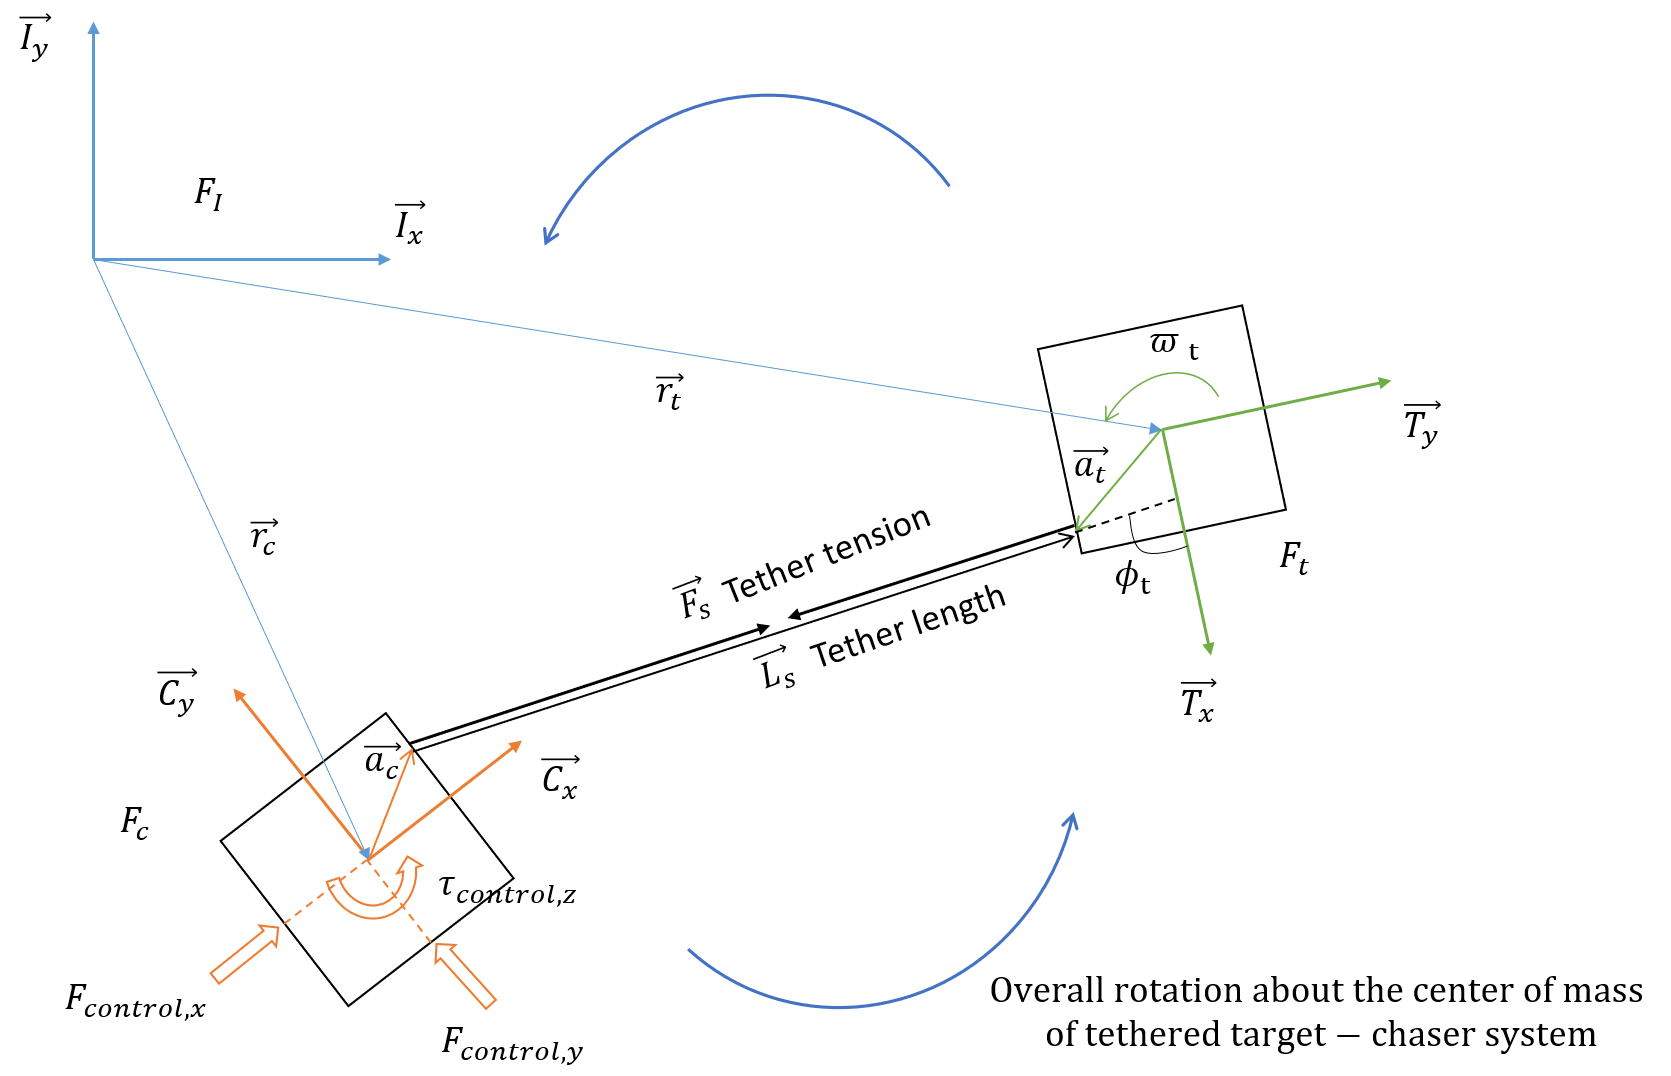
\includegraphics[width = 0.8\textwidth,right]{fig/simulation/illustration.png}
\caption{Definition of the Inertial frame, Chaser body frame and Target body coordinate systems}
\label{simu-illustration}
\end{figure}


There are three coordinate systems defined in the article and all of them are defined as right-handed system. Between two different coordinate systems the attitude matrix $A(\theta)$ is the transformation matrix which used to rotate the vector components from a body frame to Inertial frame. 
\begin{equation}
A(\theta) =
	\begin{bmatrix}
	\cos(\theta) & -\sin(\theta) \\
	\sin(\theta) & \cos(\theta)
	\end{bmatrix}
\end{equation}

	The point where tether attached the Chaser vehicle or Target vehicle is called attached point. This point is fixed in the body frame so that we can use tether attachment vector with respect to the body center of mass to describe this attach point. The tether attachment vector is denoted as $a$.
The attitude $\theta$  of a body frame ($F_C$ for the chaser or $F_T$ for of the target) is the angle of rotation between the body frame relative to the Inertial frame $F_I$ about the z-axis where the z-axis of all inertial and body frames are parallel. The transformation of vectors from body frame to Inertial frame is using the equation  $\mathbf{x_I}=A(\theta)\mathbf{x_b}$ which $I$ means Inertial frame and $b$ means body frame.
\boldmath
\begin{enumerate}

\item Reference inertial frame $F_I$ Coordinates\\		
\begin{center} $\textbf{I} =[I_x, I_y, I_z]$ \end{center}
\textbf {$F_I$} is fixed. The position of origin point and direction of three axes will not change with time.    


\item Reference inertial frame $F_T$ Coordinates\\		
\begin{center} $\textbf{T} =[T_x, T_y, T_z]$ \end{center}
\textbf{$F_T$} denotes the Target body-fixed frame. The origin point of \textbf{T} is at the center of mass of the Target vehicle. The x axis of $F_T$ is pointed to the chaser at the beginning. 

\item Reference inertial frame $F_C$ Coordinates\\		
\begin{center} $\textbf{C} =[C_x, C_y, C_z]$ \end{center}
\textbf{$F_C$} denotes the Chaser body-fixed frame.The origin point of \textbf{C} is at the center of mass of the Target. The x axis of $F_C$ is pointed to the target at the beginning. 
\end{enumerate}
\unboldmath

\section{Motion governing equation and Physics model for the system}

This section talks about the details of physical model and the motion governing equation

\subsection{Motion governing equation}

The governing equations are Newton's second law and Euler's equation.

Using the Newton's second law we can get that the sum of force vector components acting on any body in Inertia Frame,$\mathbf{F}$, equals the mass of the satellite $m$ times the resulting acceleration vector components in Inertia Frame $\ddot{r}$ i.e. $ \mathbf{F} = m\mathbf{\ddot{r}}$

Similarly, using the Euler's equation we can get that the torque of the chaser's body or target's body as a result of the force exerted by the tether and/or the chaser's control actuator equals z axis Principal moment of inertia multiplied by Angular velocity of an end-mass/satellite relative to the inertial frame (which also equals to the angular velocity relative the body frame) i.e. $J_{zz} \dot{\omega} = \tau_z$ 

\subsection{Physics model for the system}

The whole system is modeled as a nonlinear stiffness spring-damper system. The damping coefficient of the damper is constant. The tether is made of 56\% polyester and 44\% rubber. The spring constant $k$ has strong nonlinearity. 

\begin{itemize}

\item The spring constant changes as the extension of tether change 

\item When tether is extended, the spring force $F_{spring} = k\times $(length of stretched tether - tether natural length)

\item $F_{spring} = 0$ when tether is slacked

\end{itemize}

\begin{figure}[htbp]
\centering
\begin{minipage}[t]{0.48\textwidth}
\centering
\includegraphics[width=6cm]{fig/simulation/Systemmodel}
\caption{System model}
\label{simu-systemmodel}
\end{minipage}
\begin{minipage}[t]{0.48\textwidth}
\centering
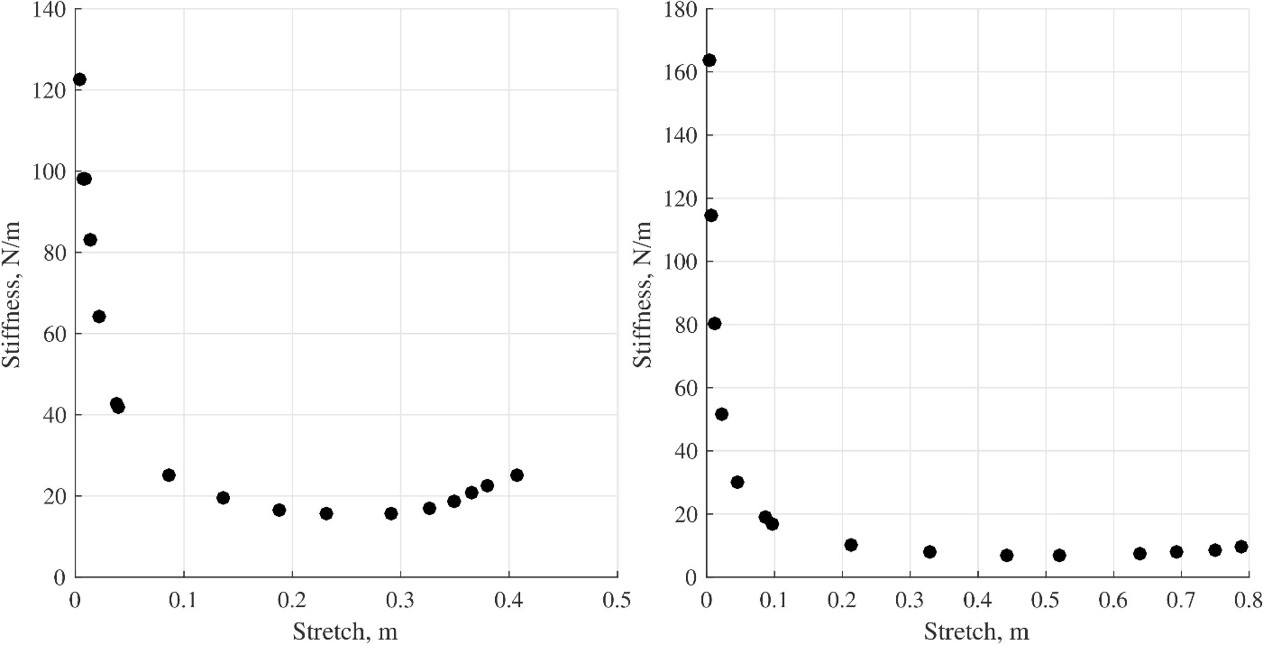
\includegraphics[width=6cm]{fig/simulation/StiffnessStetchRelation}
\caption{Stiffness stetch relation}
\end{minipage}
\end{figure}

\subsection{Force and Torque analysis}

1. For the Target vehicle, it only received the force of tether tension which denoted as $\mathbf{-\overrightarrow{F_S}}$. The torque $\tau_t$ is the torque made by tether tension about the center of mass of the target body.
\begin{equation}
\tau_t = a_{t,y}F_{s,x}^t - a_{t,x}F_{s,y}^t
\end{equation}
\quad $F_{s}^t$ is the tether force expressed in $F_t$ i.e. $F_{s}^t = A(\theta_t)^TF_S$\\
\quad\quad $F_{s,x}^t,F_{s,y}^t$ are the x and y components of $F_{s}^t$ in $F_T$, respectively.   

2. For the Chaser vehicle tether force $\mathbf{\overrightarrow{F_S}}$ and active control force $\mathbf{\overrightarrow{F_{control}}}$both exist. The torque also consists of two parts $\tau_{control}$ and  $\tau_{c}$. The $\tau_{control}$ and $\mathbf{\overrightarrow{F_{control}}}$ are the active control way that research can design in order to get the better deorbiting performance.
\begin{equation}
\tau_c = a_{c,x}F_{s,x}^c - a_{c,y}F_{s,x}^c
\end{equation}

\quad $F_{s}^c$ is the tether force expressed in $F_c$ i.e. $F_{s}^c = A(\theta_c)^TF_S$\\
\quad $F_{s,x}^c,F_{s,y}^c$ are the x and y components of $F_{s}^c$ in $F_c$, respectively.

\begin{figure}
\centering
\includegraphics[width=\textwidth]{fig/simulation/flowchart}
\caption{Flowchart of the calculation process}
\label{simu-flowchart}
\end{figure}

\subsection{Tether length, tether tension and tether torque}

According to Figure\ref{simu-illustration}, changing all the vectors in the Inertial frame then the vector form of tether length can be written as follows:

\begin{equation} \overrightarrow{L_S} = -(\overrightarrow{r_c} + A(\theta_c)\overrightarrow{a_c})+(\overrightarrow{r_t} + A(\theta_t)\overrightarrow{a_t})\end{equation}
 

As Figure \ref{simu-systemmodel} described before, the damping mechanism of tether results in the damping force: $c(\Delta\overrightarrow{v}\cdot \frac{\overrightarrow{L_S}}{\norm{\overrightarrow{L_S}}}) $. It results from damping factor times the velocity change in the tether's direction

The tether tension is: 
\begin{equation} \overrightarrow{F_S} = \bigl(k(\norm{\overrightarrow{L_S}} - L_{s,nature}) + c(\Delta\overrightarrow{v} \cdot 
	\frac{\overrightarrow{L_S}}{\norm{\overrightarrow{L_S}}})
	\bigr)
	\frac{\overrightarrow{L_S}}{
	\norm{
	\overrightarrow{L_S}
	}
	}
\end{equation}
$\frac{\overrightarrow{L_S}}{\norm{\overrightarrow{L_S}}}$ is the unit vector of the tether.$\Delta\overrightarrow{v}$ is the difference of the time derivative of two body's absolute position. 
\begin{equation}\Delta\overrightarrow{v} = \frac{d}{dt}(\overrightarrow{r_t}+A(\theta_t)\overrightarrow{a_t}) - \frac{d}{dt}(\overrightarrow{r_c} + A(\theta_c)\overrightarrow{a_c}) = \overrightarrow{v_t} + \frac{d}{dt}(A(\theta_t))\overrightarrow{a_t}-\overrightarrow{v_c}-\frac{d}{dt}(A(\theta_c))\overrightarrow{a_c}\end{equation}
Since the derivate is used for the angle, we can rewrite the $\frac{d}{dt}(A(\theta_t))\overrightarrow{a_t}$ in terms of angular rate and tether attachment vector.
\begin{equation}\frac{d}{dt}(A(\theta_t))\overrightarrow{a_t} = \frac{d}{dt}
\left(
\begin{bmatrix}
\cos(\theta_t) & -\sin(\theta_t)\\
\sin(\theta_t) & \cos(\theta_t)
\end{bmatrix} \right)
\overrightarrow{a_t} =
\begin{bmatrix}
\cos(\theta_t) & -\sin(\theta_t)\\
\sin(\theta_t) & \cos(\theta_t)
\end{bmatrix}
\left(
\begin{array}{c}
-\omega_ta_{t,y}\\
\omega_ta_{t,x}
\end{array}\right)
\end{equation}
which means that 

$$\frac{d}{dt}(A(\theta_t))\overrightarrow{a_t} = A(\theta_t)\left(
\begin{array}{c}
-\omega_ta_{t,y}\\
\omega_ta_{t,x}
\end{array}\right) \frac{d}{dt}(A(\theta_c))\overrightarrow{a_c} = A(\theta_c)\left(
\begin{array}{c}
-\omega_ca_{c,y}\\
\omega_ca_{c,x}
\end{array}\right)$$

Tether torque can be written as the time derivative of system angular momentum. It equals the time derivative of system angular momentum with regard to the relative moving coordinate system plus the moving frame's absolute angular velocity times the angular momentum. In this case the moving frame just has translational motion in Inertia frame. The moving frame's absolute angular velocity doesn't exist in this case. 
\begin{equation} M = \frac{dH}{dt} = \dot{H_{relative}} + \Omega \times H\\
		=\dot{H_{relative}} =\frac{J_{zz}\omega}{dt}= J_{zz}\dot{\omega}
\end{equation}
The torque in Inertial frame equals the torque in body frame.
For the rigid body i In the inertial frame, the Euler's equation gives us the relationship between the exerted torque $\tau$ and resulted angular acceleration $\dot{\omega}$ .i.e. 
\begin{equation}
J_i\dot{\omega} + \omega_i \times J_i\omega_i=\sum\tau
\end{equation}
According to the assumption \ref{simu-assumption} we can simplified the Euler's equation as: $J_{izz}\dot{w_{iz}}=\tau_{iz}$	i can be c for chaser or t for target.
$\tau=a_i\times F^i_S$	$\tau_t = a_{t,y}F_{s,x}^t - a_{t,x}F_{s,y}^t$	$\tau_c = a_{c,x}F_{s,x}^c - a_{c,y}F_{s,x}^c$

\section{Control goal of Chaser vehicle}
To archive the goal of deorbiting target satellite, the Chaser vehicle need to regulate and reduce the angle between tether and target so as to make the tether aligned with the target or force Chaser and target has the parallel surface. To reduce the angular rate of target vehicle, dissipate angular momentum from the system and at last make the target go to lower altitude orbit.
\begin{figure}
\centering
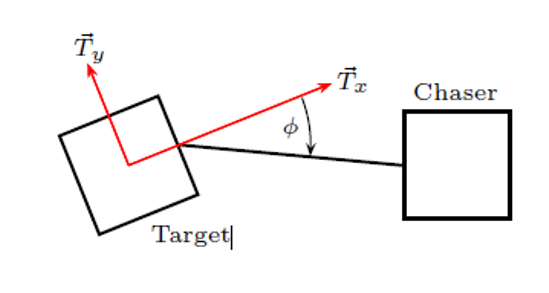
\includegraphics{fig/simulation/TetherTargetAngle}
\caption{Positive tether target angle}
\end{figure}
The easiest way is to use the proportional-derivative controller for the position and altitude control of the tether.
The force controller uses the difference between desired chaser radius vector and actual chaser radius vector as the feedback signal. The force $\overrightarrow{F_{s,control}}$ equals $\mathbf{K_P}\left[\overrightarrow{r_{des}(t)}-\overrightarrow{r_c(t)}\right]+\mathbf{K_D}\left[\overrightarrow{\dot{r_{des}(t)}}-\overrightarrow{\dot{r_c(t)}}\right]$
Similarly the torque controller uses the desired chaser attitude angle and actual chaser attitude angle as the control feedback signal.
\begin{equation}
\tau_{control} =K_{P,\theta}\left[\theta_{des}(t)-\theta_c(t)\right] + K_{D,\theta}\left[\dot{\theta_{des}(t)}-\dot{\theta_c(t)}\right]
\end{equation}

$K_P,K_{P,\theta},, K_D,K_{D,\theta}$ are the Proportional gain matrix and the Derivative gain matrix respectively. These matrix value are designed and tuned by designer for the special case.

\section{MATLAB Implementation}
In this section, the MATLAB simulation case \ref{appendix-thruststab} is implemented. To simplified the study, the implementation case use only one controller. The thrust stabilization only use force controller. The Tether Satellite System Spin Stabilization only use torque control, commanding the chaser to continually point its $C_x$  axis toward the target. In the real case the controller can be the combination of these two kinds. Here we just implemented the Thrust stabilization of single tether for illustration the problem.

The detail MATLAB code is in the Appendix. Symbols have the same meaning and constant values are not changed, as\cite{hovell2017experimental}. 

\subsection{Thrust stabilization}
The chaser is designed as uniformly accelerated motion for simplicity. The motion can be replaced by any other arbitrarily defined motion.
\begin{equation}
\overrightarrow{r_{des}(t)}=\overrightarrow{r_0}+\overrightarrow{d}\frac{t^2}{2}
\end{equation} d is the acceleration got from the desired final radius vector, the initial radius vector and assigned time for motion, $\overrightarrow{d} = \frac{2(\overrightarrow{r_{final}}-\overrightarrow{r_0})}{t^2}$, $\overrightarrow{\dot{r_{des}}(t)}=\overrightarrow{d}t$ 
\begin{figure}[htbp]
\centering
\begin{minipage}[t]{0.48\textwidth}
\centering
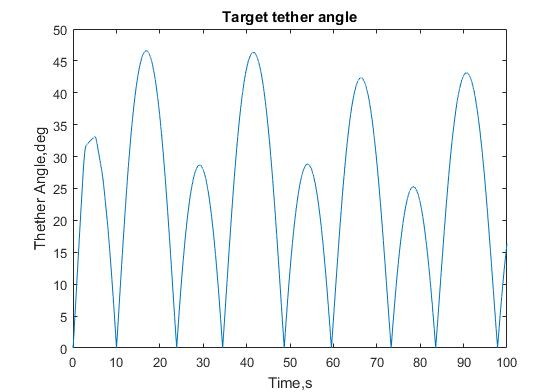
\includegraphics[width=6cm,height=6cm]{fig/simulation/ThrustStable/Targettetherangle.jpg}
\end{minipage}
\begin{minipage}[t]{0.48\textwidth}
\centering
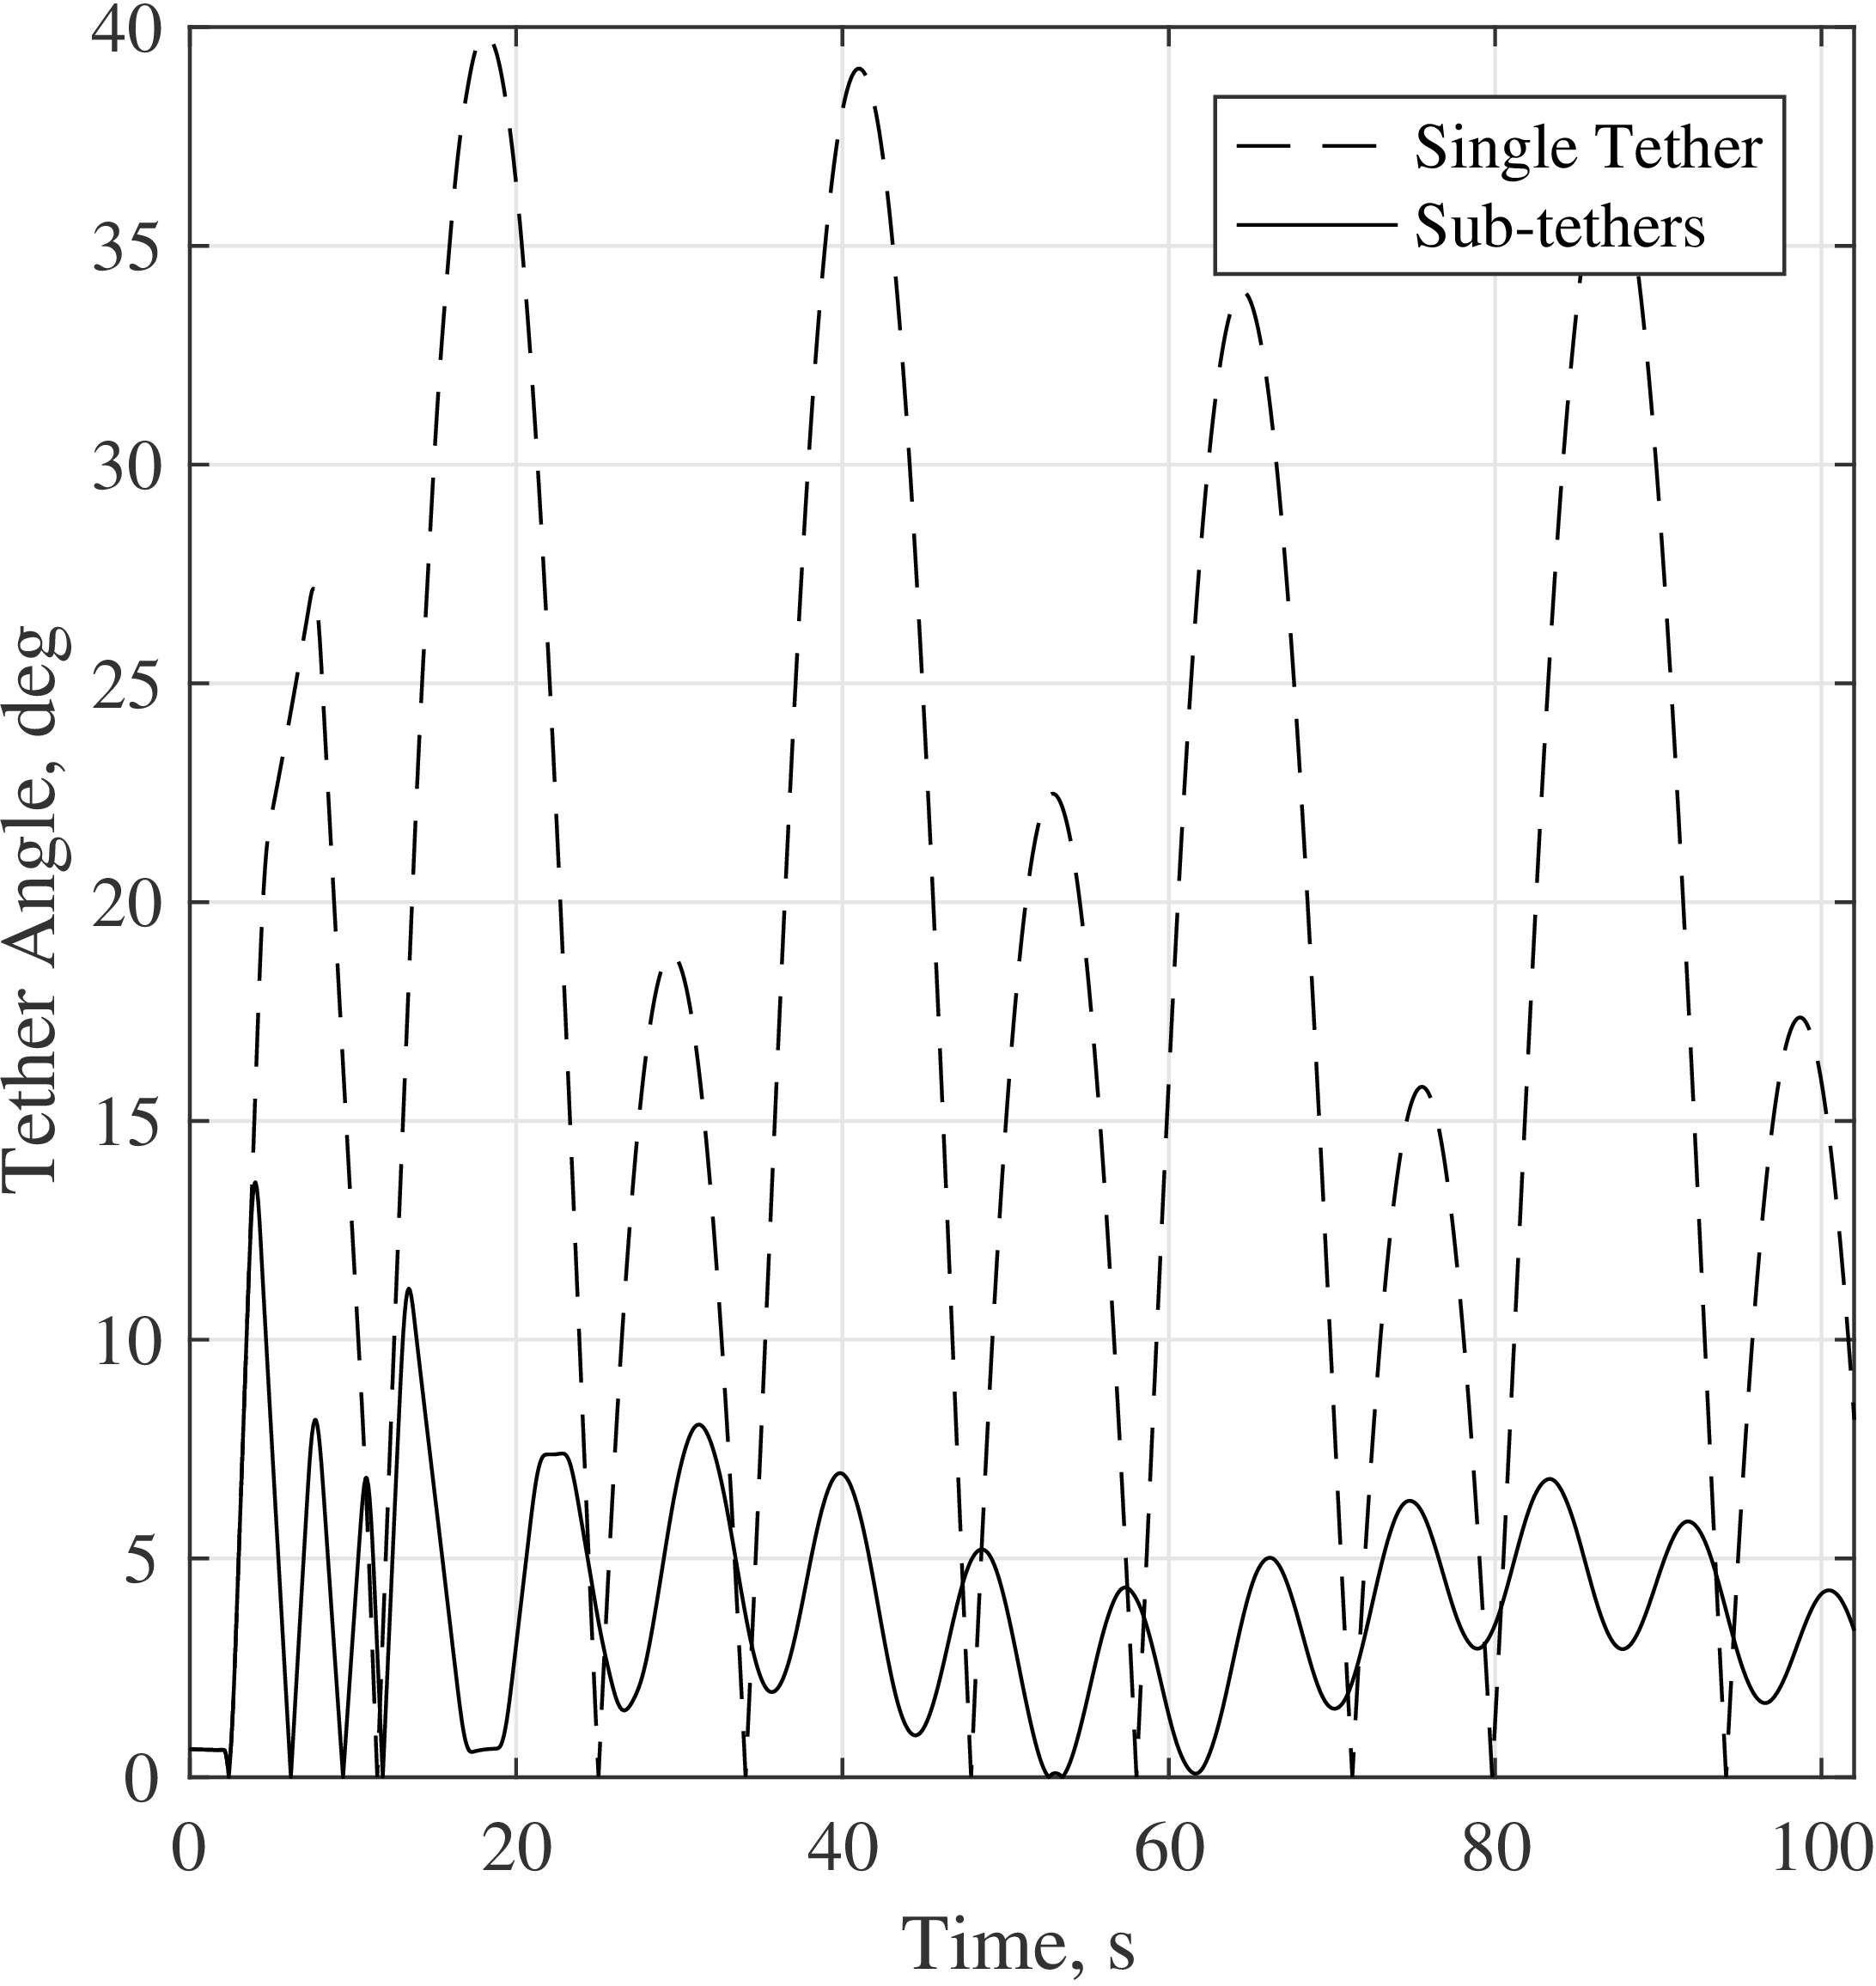
\includegraphics[width=6cm,height=6cm]{fig/simulation/ThrustStable/Targettetheranglesample.jpg}
\end{minipage}
\caption{Comparison of Target tether angle. Left: Kaiwen	Right: Hovell}
\end{figure}
\begin{figure}[htbp]
\centering
\begin{minipage}[t]{0.48\textwidth}
\centering
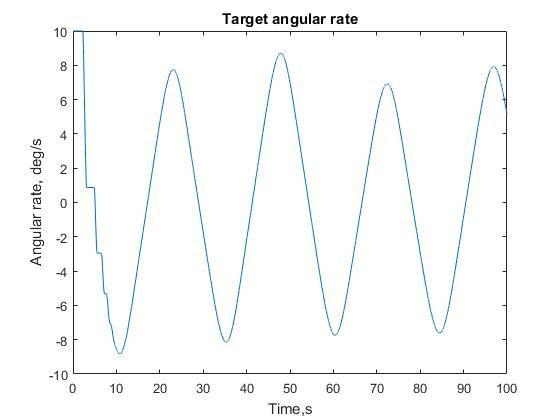
\includegraphics[width=6cm,height=6cm]{fig/simulation/ThrustStable/Targetangularrate.jpg}
\end{minipage}
\begin{minipage}[t]{0.48\textwidth}
\centering
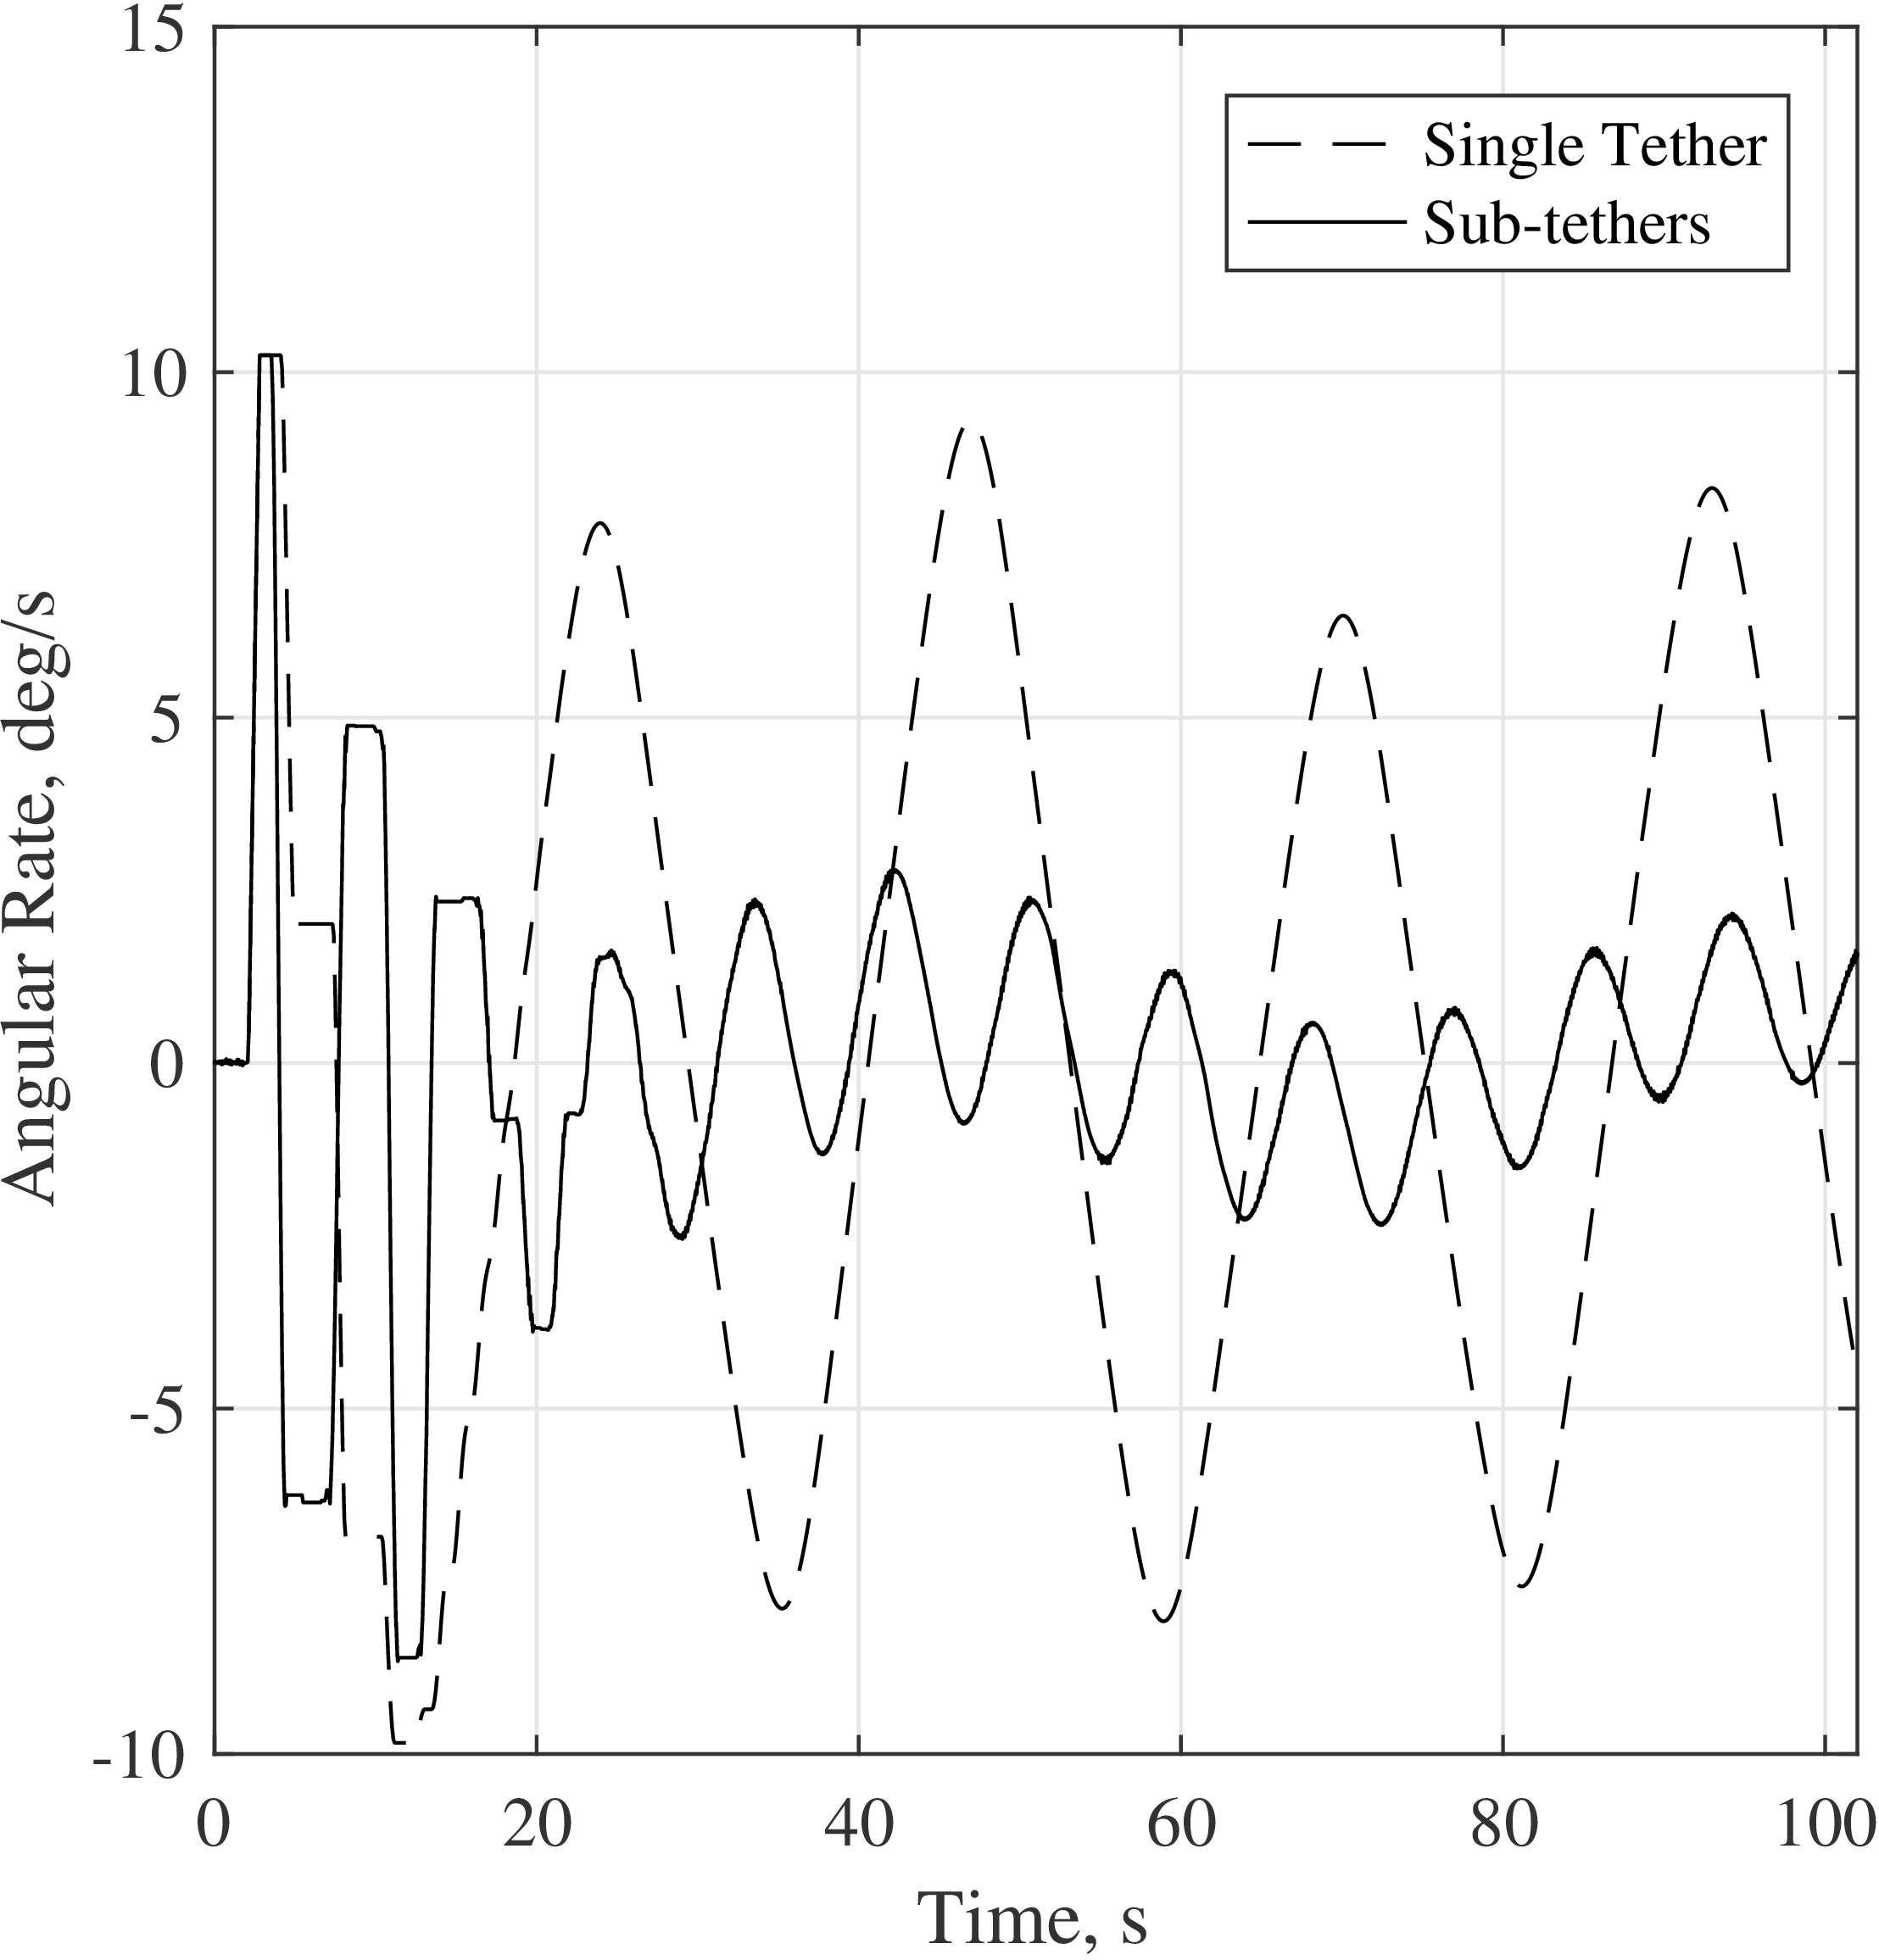
\includegraphics[width=6cm,height=6cm]{fig/simulation/ThrustStable/Targetangularratesample.jpg}
\end{minipage}
\caption{Comparison of Target angular rate.		Left: Kaiwen	Right: Hovell}
\end{figure}
\begin{figure}[htbp]
\centering
\begin{minipage}[t]{0.48\textwidth}
\centering
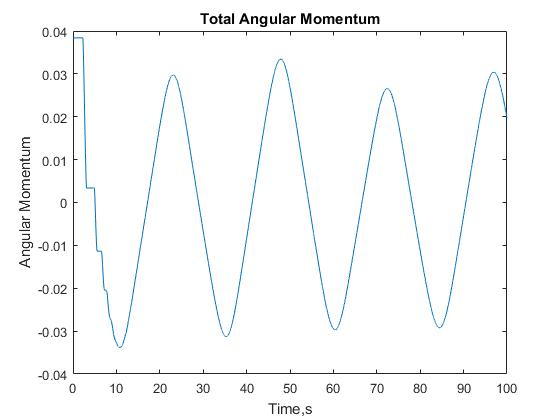
\includegraphics[width=6cm,height=6cm]{fig/simulation/ThrustStable/Totalangularmomentum.jpg}
\end{minipage}
\begin{minipage}[t]{0.48\textwidth}
\centering
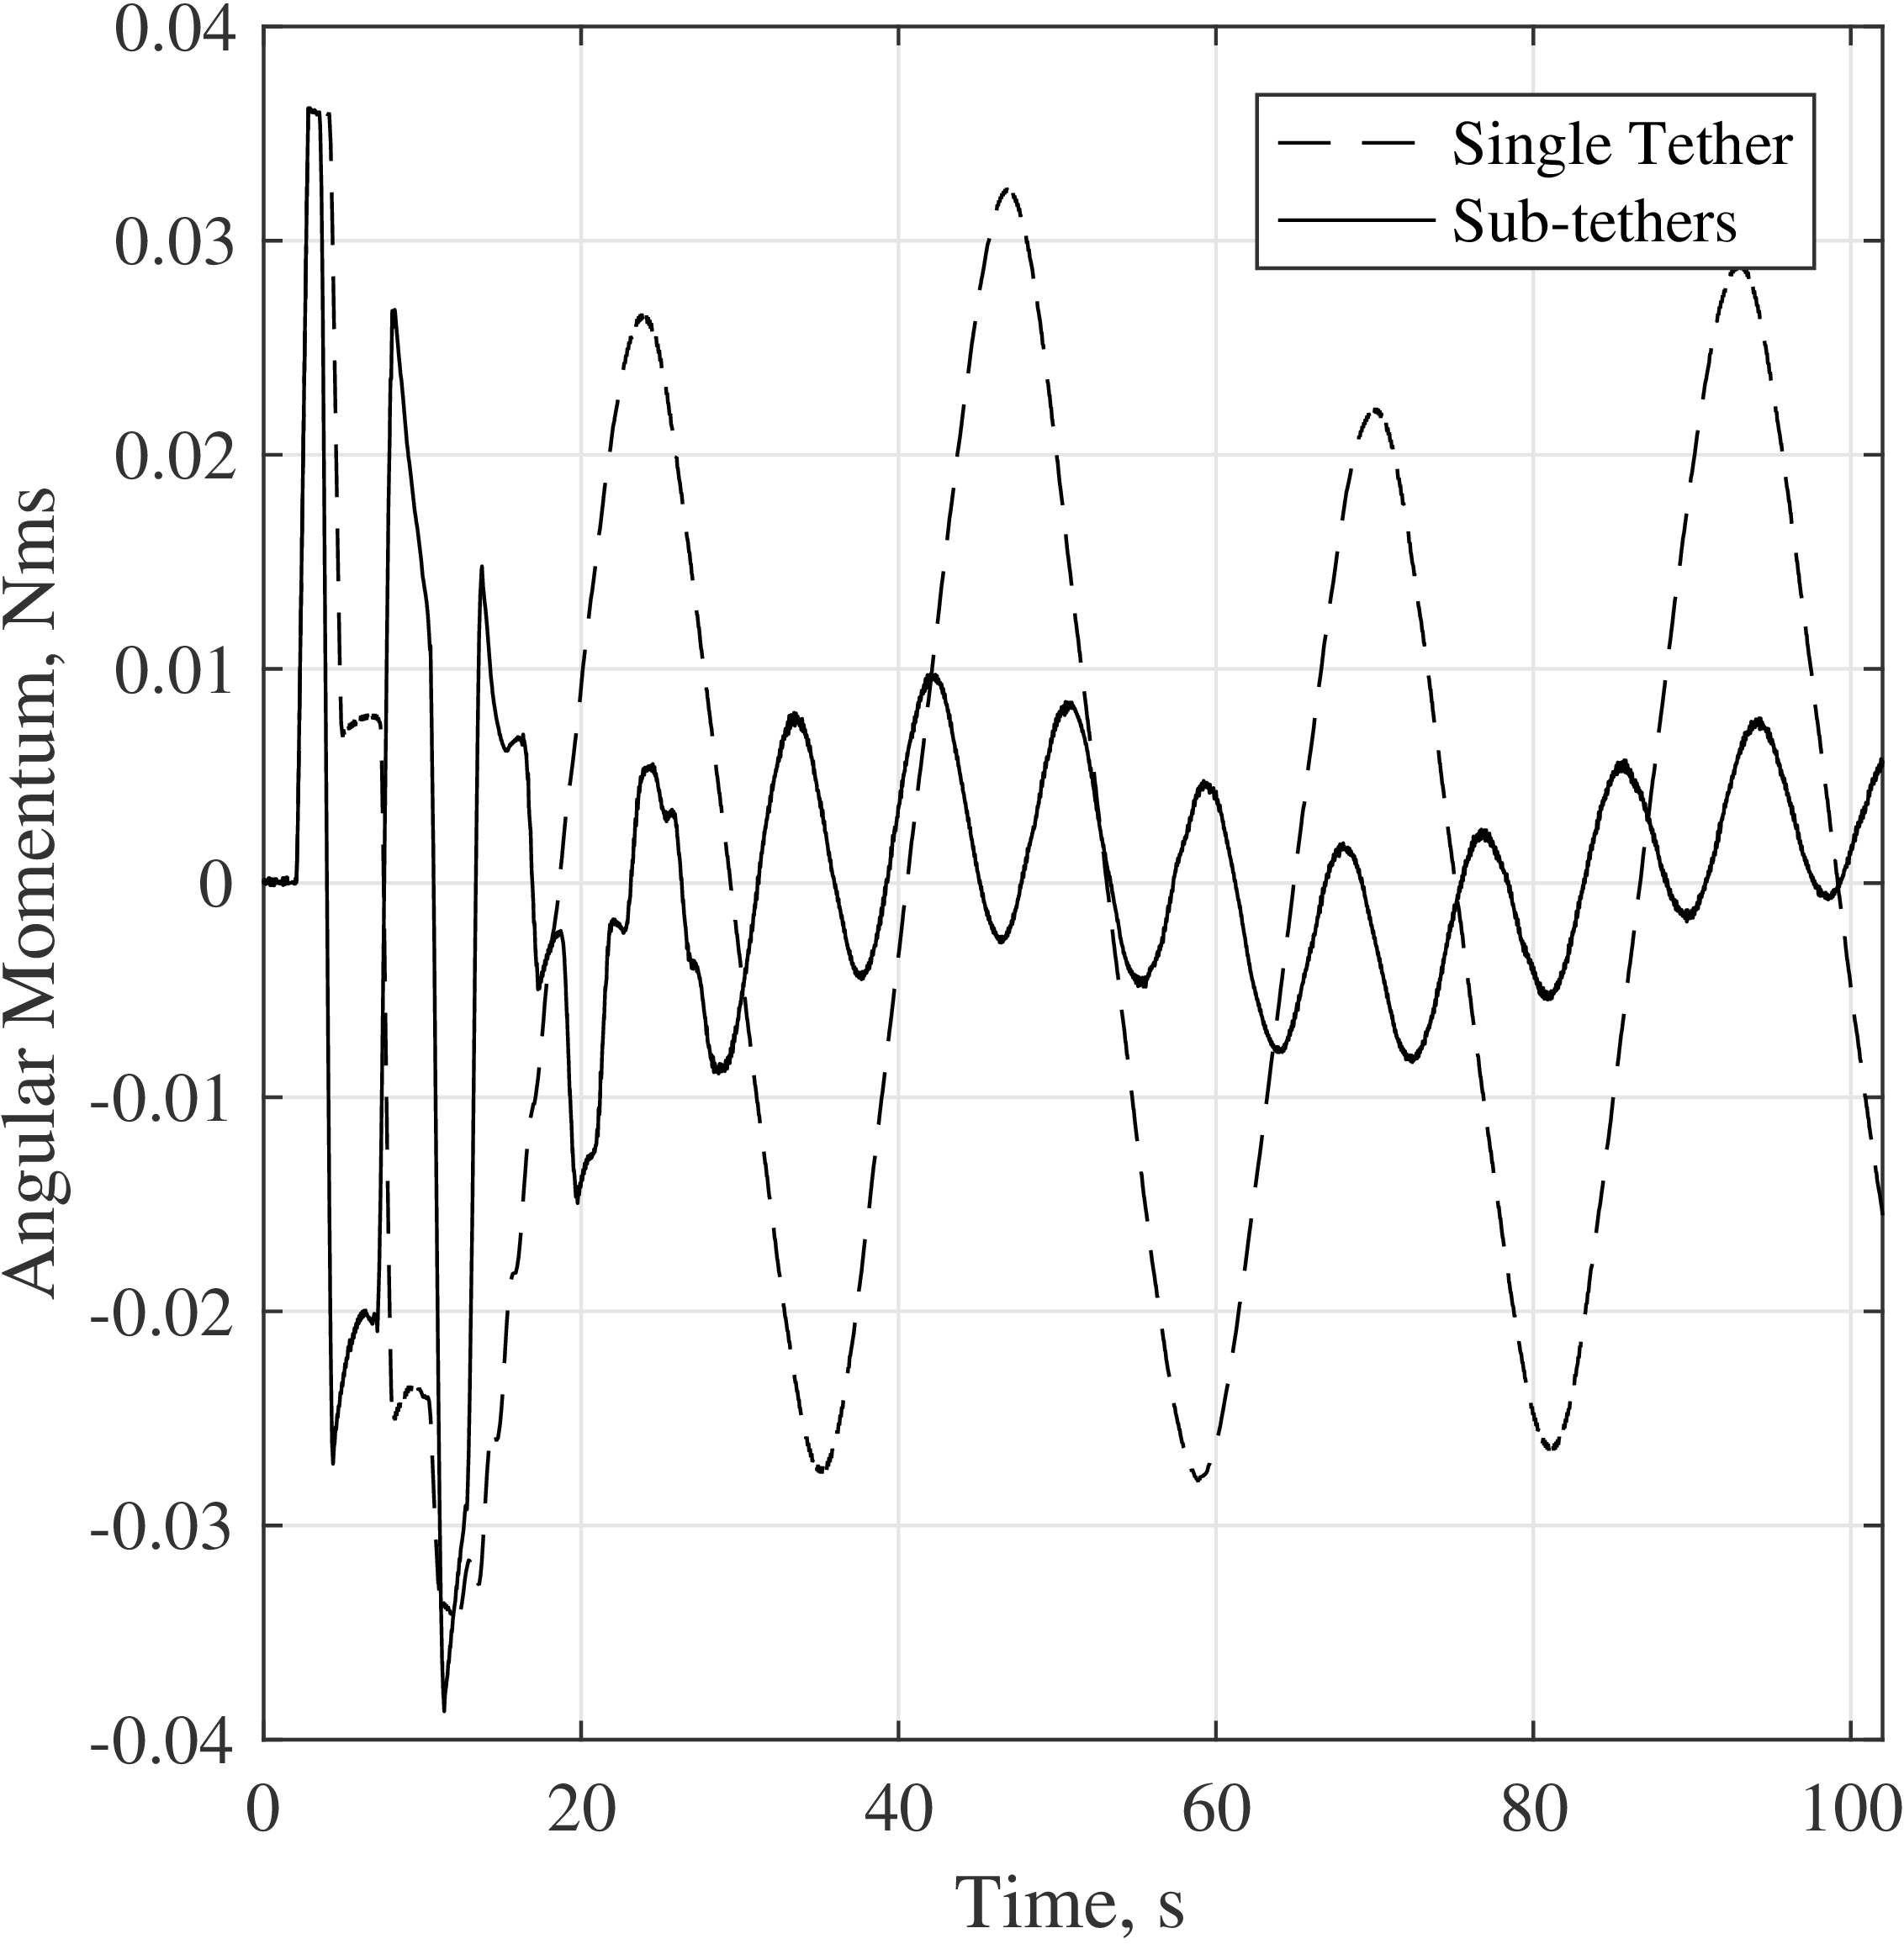
\includegraphics[width=6cm,height=6cm]{fig/simulation/ThrustStable/Totalangularmomentumsample.jpg}
\end{minipage}
\caption{Comparison of Total angular momentum.		Left: Kaiwen	Right: Hovell}
\end{figure}
\begin{figure}[htbp]
\centering
\begin{minipage}[t]{0.48\textwidth}
\centering
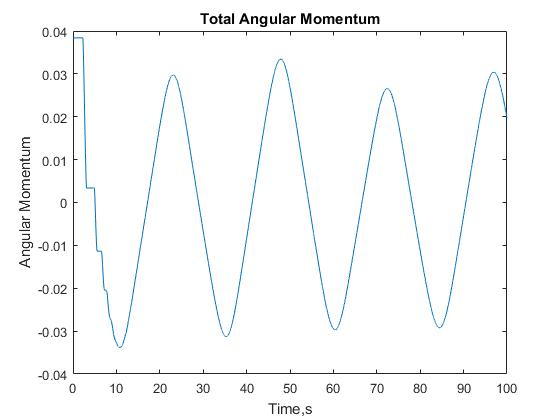
\includegraphics[width=6cm,height=6cm]{fig/simulation/ThrustStable/Totalangularmomentum.jpg}
\end{minipage}
\begin{minipage}[t]{0.48\textwidth}
\centering
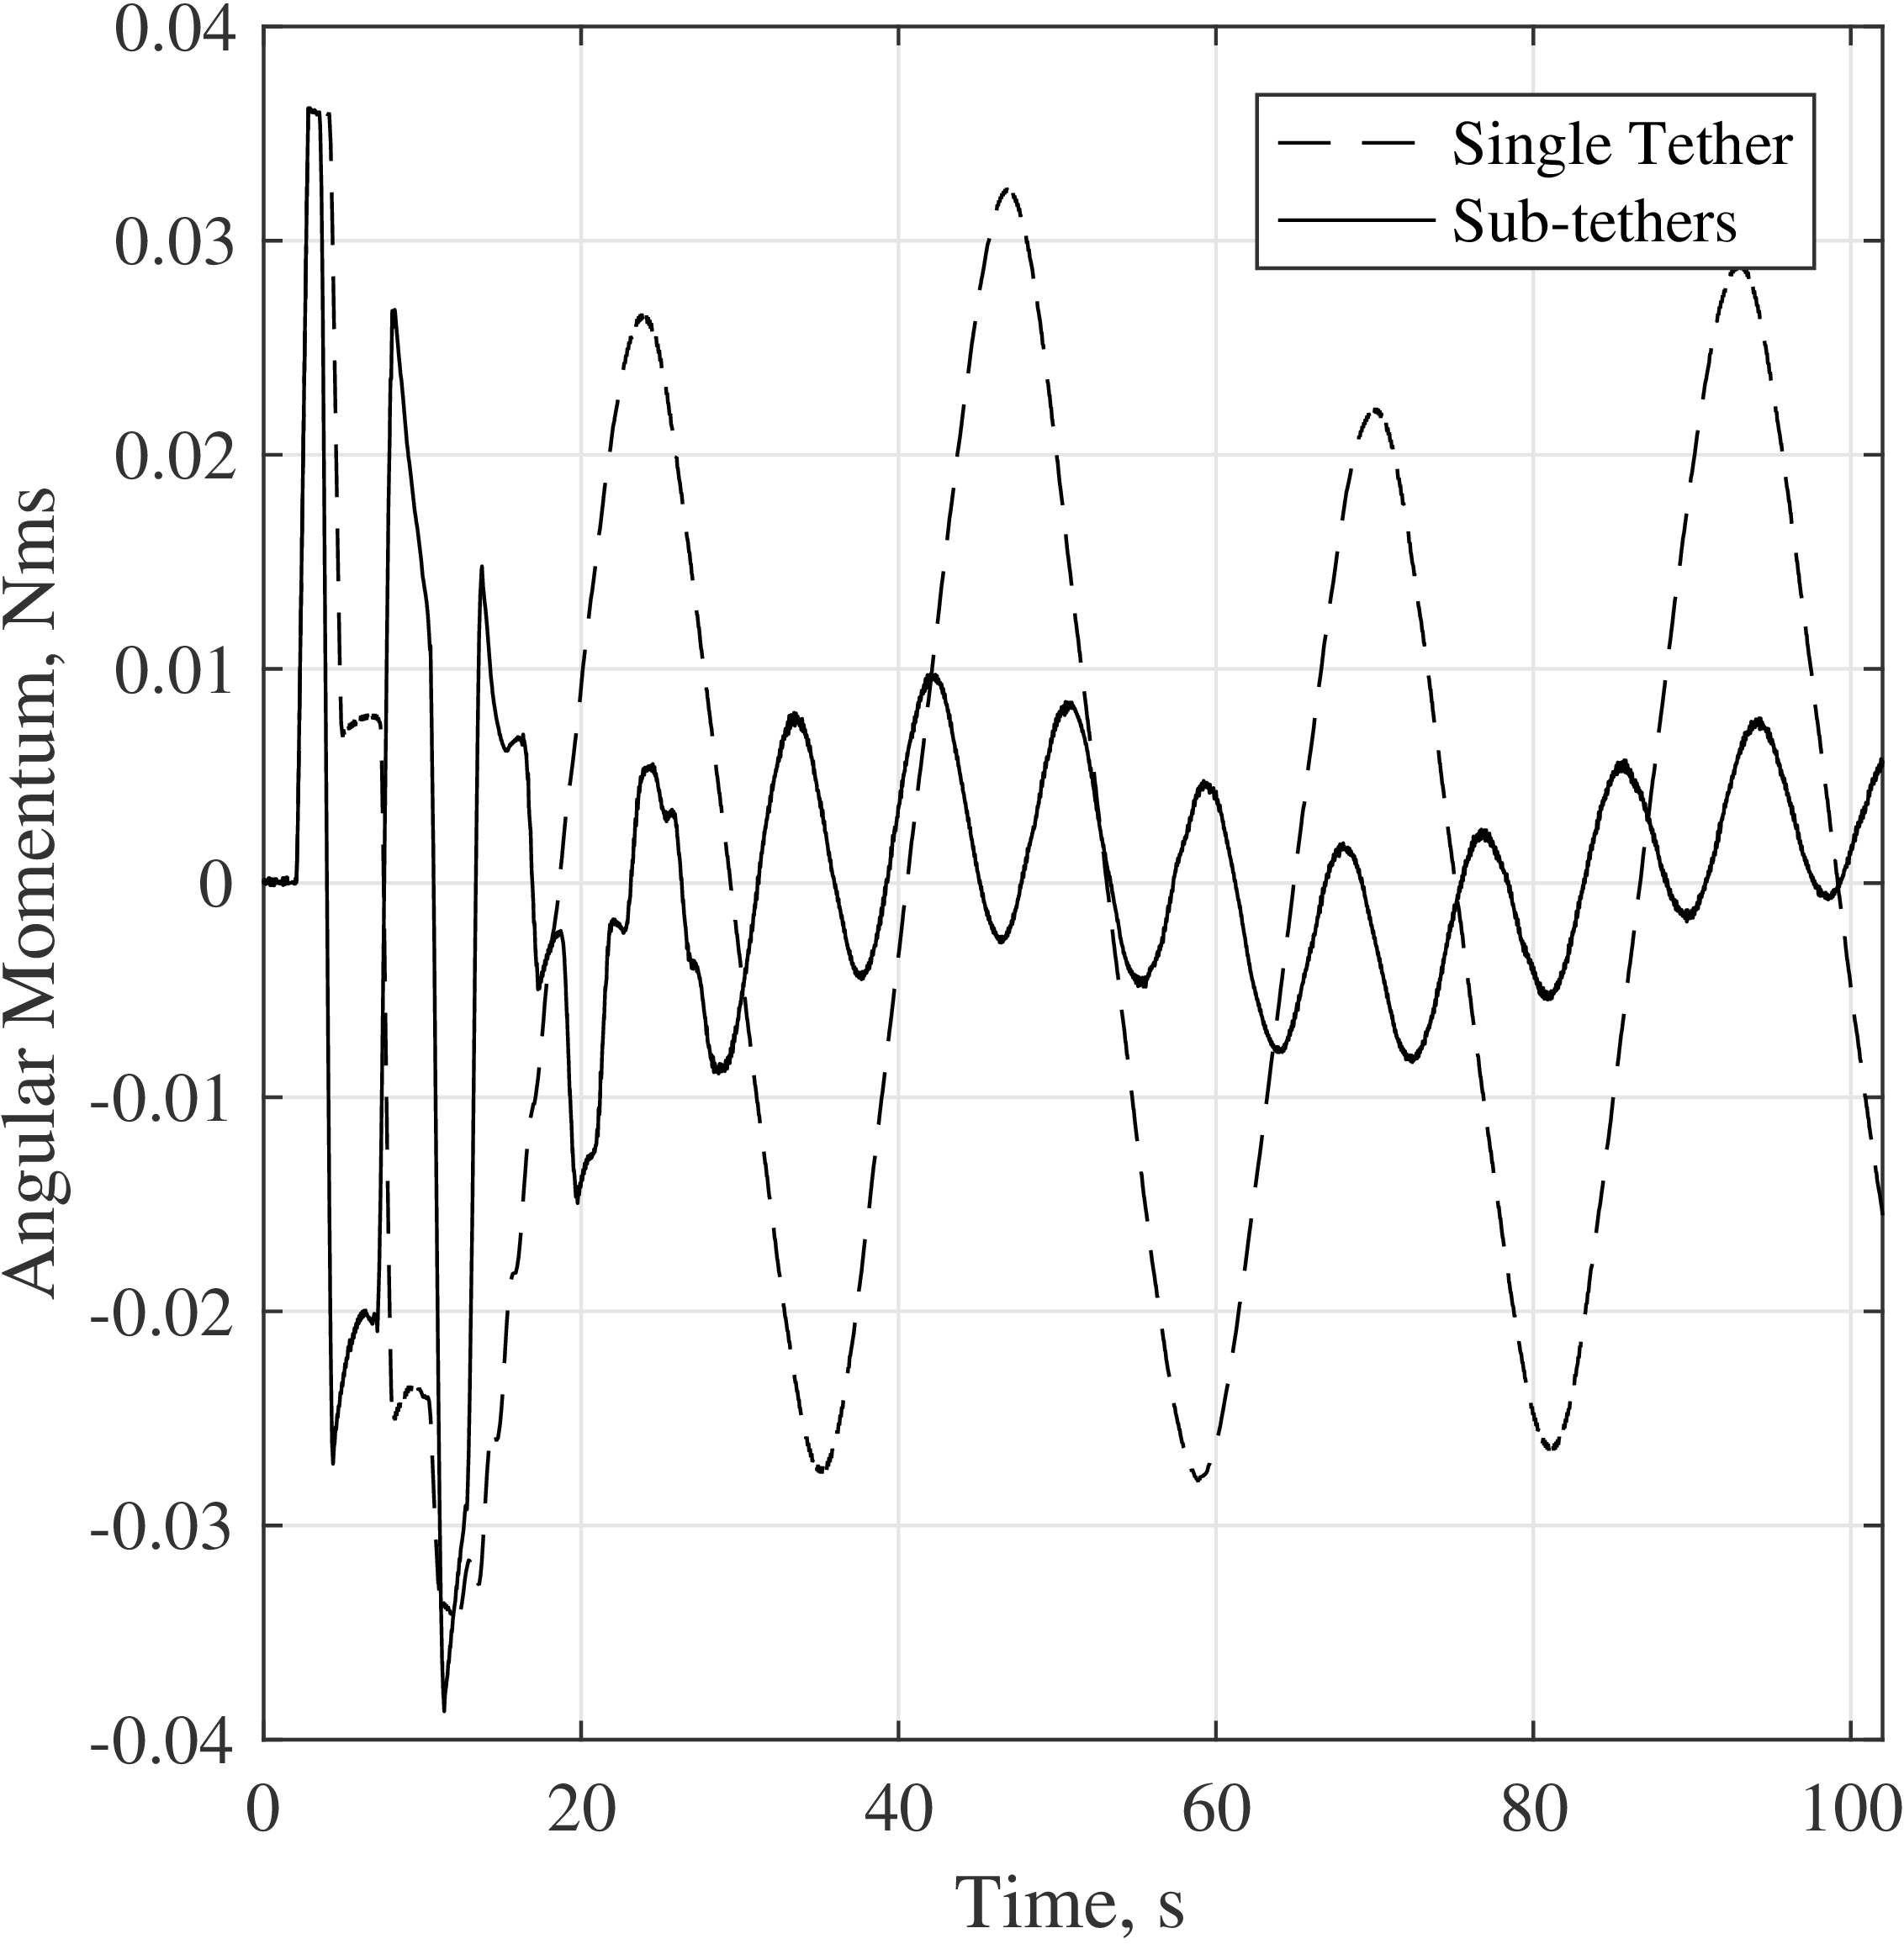
\includegraphics[width=6cm,height=6cm]{fig/simulation/ThrustStable/Totalangularmomentumsample.jpg}
\end{minipage}
\caption{Comparison of Total angular momentum.		Left: Kaiwen	Right: Hovell}
\end{figure}
\begin{figure}[htbp]
\centering
\begin{minipage}[t]{0.48\textwidth}
\centering
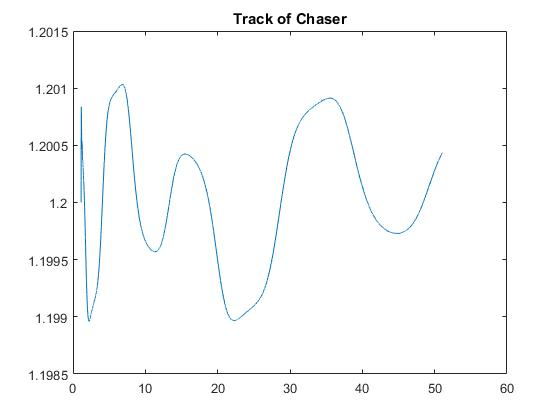
\includegraphics[width=6cm,height=6cm]{fig/simulation/ThrustStable/TrackofChaser.jpg}
\caption{Track of Chaser}
\end{minipage}
\begin{minipage}[t]{0.48\textwidth}
\centering
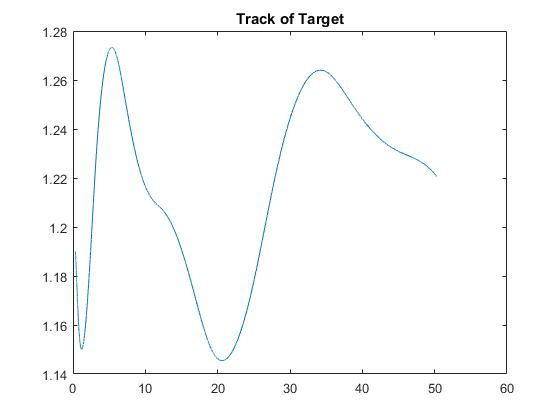
\includegraphics[width=6cm,height=6cm]{fig/simulation/ThrustStable/Trackoftarget.jpg}
\caption{Track of Target}
\end{minipage}
\end{figure}
From the figure comparison, we know that the effect of implementation is quite well.
\newpage
